%!TEX root = ../main.tex
\section{Geometric camera model}
\label{sec:camera-model}

We first present the geometric camera model used in this chapter. 
%As explained below, our simplified model represents the camera using the focal length $f_\mathrm{px}$, pitch $\theta$ and roll $\psi$ angles.
Under the pinhole camera model, the pixel coordinates $\mathbf{p}_\mathrm{im}$ of a 3D point $\mathbf{p}_\mathrm{w}$ are given by
%
\begin{equation}
\mathbf{p}_{\mathrm{im}} = [\lambda u \; \lambda v \; \lambda]^T = \mathbf{K} \left[\mathbf{R} | \mathbf{t}\right] \left[ \mathbf{p}_{\mathrm{w}} | 1 \right]^T
\end{equation}
%
in homogeneous coordinates, where $\mathbf{K}$ is the camera projection matrix (camera intrinsics), $\mathbf{R}$ and $\mathbf{t}$ are the camera rotation and translation in the world reference frame (camera extrinsics). Simplifying the model further to square pixels, no skew, and image center at the principal point, the projection matrix $\mathbf{K}$ is given by $\mathbf{K} = \mathrm{diag}([f \; f \; 1])$, where $f$ is the focal length in pixels. We further assume the camera to be at the origin by using $\mathbf{t} = \left[0, 0, 0\right]^T$. 

Since the camera parameters are to be estimated from a single image, we first express them as a function of image features. Let us first consider the focal length $f$. Since it has no direct interpretation in the image, we instead estimate the vertical field of view $h_\theta$, a more intuitive measure: 
%
\begin{equation}
h_{\theta} = 2 \arctan \left( \frac{ h }{ 2f } \right) \,,
\end{equation}
%
where $h$ is the image height.

We next consider the rotation matrix $\mathbf{R}$, which can be parameterized by roll $\psi$, pitch $\theta$, and yaw $\varphi$ angles. There exists no natural reference frame to estimate $\varphi$ (left vs right) from an arbitrary image. Therefore, we constrain the rotation to only pitch and roll components, simplifying the extrinsic rotation matrix to $\mathbf{R} = \mathbf{R}_z(\psi) \mathbf{R}_x(\theta)$. We can use the horizon line as an intuitive representation for these angles. As in~\cite{Workman2016}, we define the horizon line offset $\rho$ as the perpendicular distance between the horizon and the center of the image. This offset can be derived from pitch angle $\theta$, roll angle $\psi$ and focal length $f$ as 
%
\begin{equation}
\rho = \frac{2 f \tan\theta}{\sqrt{\tan^2\left( \psi \right) + 1}} \,.
\label{eq:horizon_offset}
\end{equation}
%

%We define the horizon line midpoint $b_{\mathrm{p}}$ as the $y$-coordinate of its intersection with the vertical axis in the image and roll $\psi$ with respect to horizontal.

%The midpoint $b_{\mathrm{p}}$ can be derived from pitch angle $\theta$ and focal length $f_{\mathrm{px}}$ as
%
%\begin{equation}
%b_{\mathrm{p}} = 2 f_{\mathrm{px}} \tan\theta \,.
%\label{eq:horizon_midpoint}
%\end{equation}
%
In this image units representation, the top and bottom of the image have coordinates 1 and $-1$ respectively. 

Throughout this chapter, camera calibration refers to the vertical field of view $h_{\theta}$, roll $\psi$ (also called slope) and offset $\rho$ from this simplified geometric camera model. A summary of these parameters is shown in fig.~\ref{fig:camera_parameters_summary}.

\begin{figure}
\centering
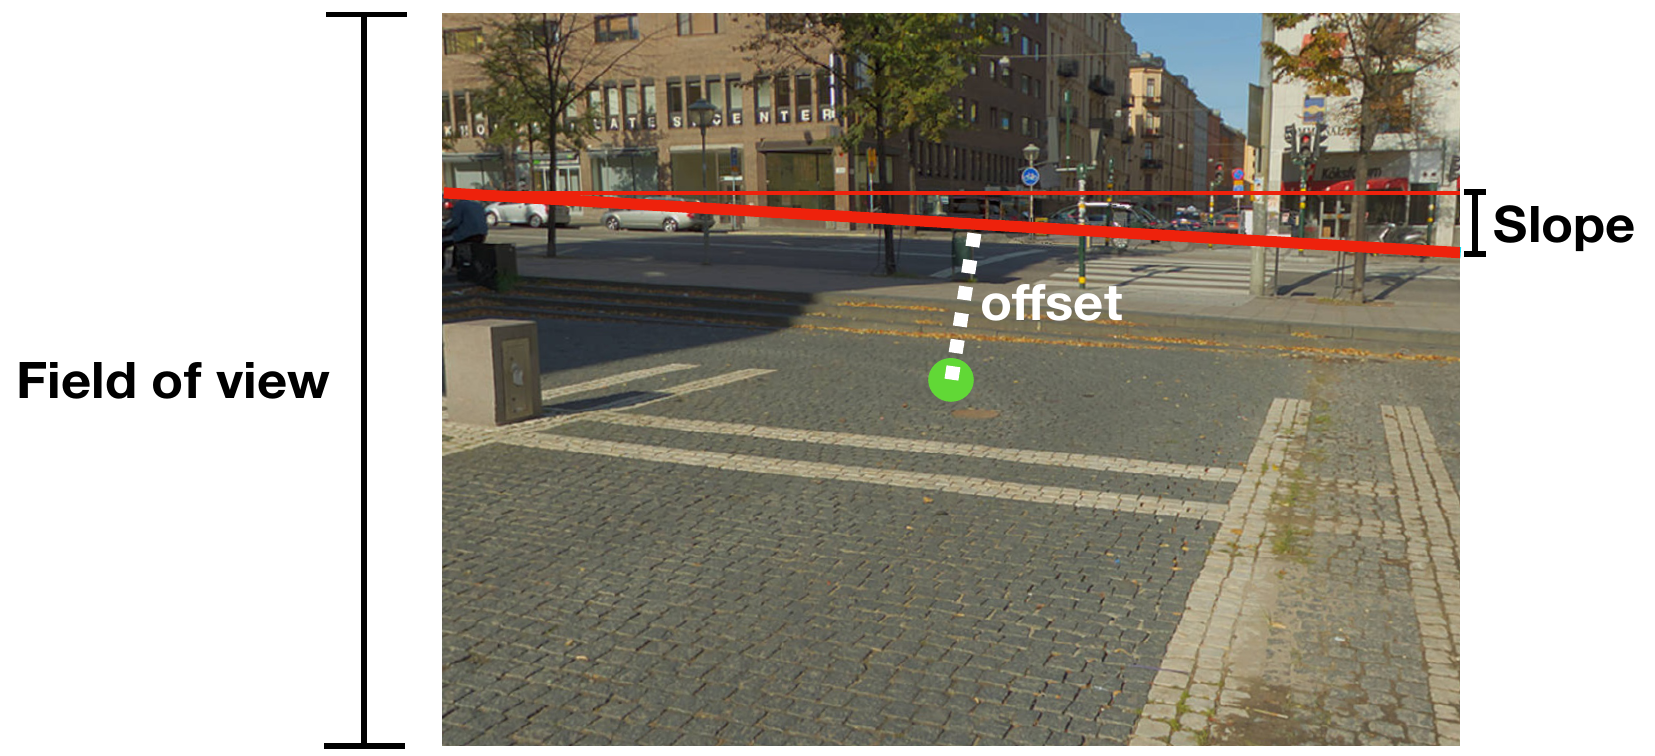
\includegraphics[width=\linewidth]{figures/cvpr18_parameters.png}
\caption[Camera parameters]{Representation of the three parameters used to represent camera calibration in image space.}
\label{fig:camera_parameters_summary}
\end{figure}
